\documentclass[fleqn,12pt]{article}
\usepackage{tikz}
\usepackage{bigpage,graphicx,scalalistings}
\usepackage{questions}

\def\topfraction{0.9}
\def\floatpagefraction{0.85} 

\def\Programming{\textbf{[Programming]}}
\def\scalacolour{\color{blue}}

%\questionsonly
%\questionsandanswers
%\answersonly
%\nontuteanswersonly

\title{Concurrent Programming: Exercise Sheet 1}
\author{Gavin Lowe}

\sloppy

\begin{document}
\maketitle

You should complete all questions marked \Programming\ at a computer.
%, and include suitable testing code with your answers.

Questions marked $\dagger$ will not normally be discussed in class.  Model
answers are included below.  You should attempt these questions and mark them
yourself; ask your tutor if they would like them to be handed in.

Some of the early questions in this sheet are designed to help you understand
how hard ill-disciplined programs are to understand.  

%\makeqnta{body1}
\makeqa{body1}

%\questionsoff\nontuteanswersoff\begin{nontutequestion}
Consider a web browser that supports multiple tabs (i.e.~different
tabs for different web pages).  Why might it be beneficial to use
concurrency in the implementation of such a web browser?  Would this
still make sense on a uni-processor computer?  What problems might
arise from such a design?
\end{nontutequestion}

%%%%%

\begin{nontuteanswer}
There are two main reasons: ease of implementation, and efficiency.

Building a web browser this way is easier!  The different tabs are largely
independent.  It's far easier to write a thread that deals with a single tab,
and run $n$ such threads, than to write a single thread that deals with all
$n$ tabs.  Each tab thread will probably need to interact with some main
browser thread, but that's relatively straightforward.

In terms of efficiency, concurrency might be used to give better response to
user actions (i.e.\ lower latency), and better overall performance (i.e.\
higher throughput); of these, the former seems more important.

As an example of why a sequential implementation might be unsatisfactory,
consider a user who has two tabs open, one viewing a page that automatically
re-loads every few minutes, and another that the user is actively reading.
Suppose the user tries to scroll down in the second page just after the first
page starts a re-load; then the user has to wait until the re-load completes
before the second page scrolls; this could take several seconds, and so annoy
the user.  (The Firefox browser used to act in this way.)  If the different
tabs used different processes, then they could run concurrently so the user
wouldn't see this delay.  This would still be the case on a uni-processor
machine: the fact that the two processes are competing for the processor would
slow things down a bit, but probably not enough for the user to notice.

The problem is, of course, that two processes might try to access some shared
data (e.g.~the history list) simultaneously, leading to race conditions.
These race conditions can be avoided by careful programming: see the rest of
the course!
\end{nontuteanswer}
 % Why make a web browser use concurrency?  

%\begin{nontutequestion}
Suppose process \SCALA{P} performs $m$ atomic actions (sequentially), and
process \SCALA{Q} performs $n$ atomic actions (sequentially).  When \SCALA{P}
and \SCALA{Q} are run in parallel, how many interleavings of atomic actions
are there?
\end{nontutequestion}
%
\begin{nontuteanswer}
There are a total of $m+n$ atomic actions.  The number of ways of choosing
which $m$ of these belong to~\SCALA{P} is
\[
\left( \begin{array}{@{}c@{}} m+n \\ m \end{array} \right) =
\frac{(m+n)!}{m! n!}
\]
\end{nontuteanswer}

 % Count number of execution seqs - formula

%\begin{question}
Consider the code below.
%
\begin{scala}
var x = 0

def p = proc{ x = x+1; x = x+2 }

def q = proc{ x = x+4 }

def system = p || q
\end{scala}
%
Suppose the atomic actions are reading or writing a variable.
When \SCALA{system} is run, what are the possible final values of \SCALA{x}?
Draw a diagram to illustrate the different possible execution paths.
\end{question}
%
\begin{answer}
The diagram below shows all interleavings until one process terminates, at
which point the system becomes deterministic.  Each label is a triple: the
process doing the event ($P$ or $Q$); an indication of the action (``r'' for
read or ``w'' for write); and the value read or written.  The figures in
circles then show the final value of \SCALA{x} that will result.  The possible
values are 3, 4, 5, 6, 7.  As a check, the diagram shows 
\( {\scriptstyle
  \left( \begin{array}{@{}c@{}} \scriptstyle 6 \\[-1mm] \scriptstyle
    4 \end{array} \right)} = 15 \) interleavings.
%
\begin{center}
\ 
\includegraphics[width=12cm]{interleavings2.eps}\ 
\end{center}
%
The point is that even a very simple program with dependent atomic actions can
become very difficult to understand. 
\end{answer}
 % based on Andrews 2.10; results of particular
                       % interleaving 

%% based on Andrews 2.15
\begin{question}
Consider the code below.
%
\begin{scala}
var x = 0; var y = 10

def p = proc{ while(x != y) x = x+1 }

def q = proc{ while(x != y) y = y-1 }

def system = p || q
\end{scala}
%
Will the process \SCALA{system} terminate?  Explain your answer.
\end{question}
%
\begin{answer}
It might or might not terminate.

Consider an execution where we reach a state with \SCALA{x=4} and \SCALA{y=5},
both processes evaluate \SCALA{x!=y} in this state and enter the body of the
loop.  Now suppose each loop body is executed, giving \SCALA{x=5} and
\SCALA{y=4}.  Subsequently we always have \SCALA{x>y}, so neither process
terminates.

Alternatively, again suppose we reach a state with \SCALA{x=4} and
\SCALA{y=5}, both processes evaluate \SCALA{x!=y} in this state and enter the
body of the loop.  Now suppose \SCALA{p} runs, setting \SCALA{x=5}, evaluates
the guard which is now true, and terminates.  However, when \SCALA{q} runs, it
sets \SCALA{y=4}, so never terminates.  Similarly, it is possible
for~\SCALA{q} to terminate, but not~\SCALA{p}.

There are also problems that are caused by the use of caching.  For example,
|p| could reach a state with |x = 6|, while working with |y = 10| in its
cache; and |q| could reach a state with |y = 4|, while working with |x = 0| in
cache.  When they do refresh their caches, they will again run forever.  


It is easy to find executions where both terminate.
\end{answer}
 % based on Andrews 2.15

{\setnontutequestion\begin{question}
Consider an object representing a bank account, from the following class.
%
\begin{scala}
class Account{
  private var balance = 0

  def credit(value: Int) = atomically{ balance += value }

  def canDebit(value: Int): Boolean = atomically{ balance >= value }

  def debit(value: Int) = atomically{ balance -= value }
}
\end{scala}
%
The ``|atomically|'' pseudocode is intended to indicate that each
procedure is performed atomically (we will see how to do this in a
later chapter).

A process that wants to perform a debit should first of all call
\SCALA{canDebit}, to avoid the account from going overdrawn; for example
%
\begin{scala}[showstringspaces=false]
  if(account.canDebit(value)) account.debit(value)
  else println("Debit not allowed!")
\end{scala}

What can go wrong if two processes execute the above code at the same
time?  Sketch a solution to this problem.
\end{question}

%%%%%

\begin{answer}
Suppose the current balance is 100, and both processes want to debit 100;
clearly only one should succeed.  Both processes could call
\SCALA{canDebit(value)}, getting back the result \SCALA{true}.  They would
then both call \SCALA{debit}, leading to the account balance becoming $-$100.
This is a time-of-check to time-of-use (TOCTTOU) problem: the check that there
is enough money in the account is no longer valid when the debit is
performed. 

The point is that the \SCALA{canDebit} action of one process and the
\SCALA{debit} action of the other are not independent.  This leads to a race
condition.

The obvious way to avoid this problem is to combine the \SCALA{canDebit} and
\SCALA{debit} actions into a single atomic action within the \SCALA{Account}
class.  Something like
%
\begin{scala}
/** Attempt to debit value.  Return true if successful. */
def tryDebit(value: Int): Boolean = atomically{
  if(balance >= value){ balance -= value; true } else false
}
\end{scala}
% 
The calling code (outside the |Account| class) can do the right thing with the
boolean result. 
\end{answer}

} % Account with race condition.

\begin{question}
\begin{figure}
\begin{scala}
class Queue[A]{
  /** A node in the linked list. */
  private class Node(val datum: A, var next: Node)

  /** The dummy header node. */
  private var head = new Node(null.asInstanceOf[A], null)

  /** The last node in the list. */
  private var last = head

  /** Is the queue empty? */
  def isEmpty = last == head

  /** Add x to the queue. */
  def enqueue(x: A) = {
    val node = new Node(x, null); last.next = node; last = node
  }

  /** Dequeue a value.  Pre: the queue is not empty. */
  def dequeue: A = {
    require(!isEmpty); head = head.next; head.datum
  }
}
\end{scala}
\caption{A sequential queue based on a linked list.}
\label{fig:queue}
\end{figure}

Figure~\ref{fig:queue} gives the implementation of a queue based on a linked
list.  The implementation is correct when the queue is used sequentially.
However, if the queue is used concurrently (i.e.~with two or more threads
calling the operations concurrently), then it can go wrong in a number of
different ways.  
%
%I have spotted six essentially different ways in which it can go wrong.
Describe as many as possible essentially different ways in which it can go
wrong (I have spotted six essentially different ways).
%
For the purposes of this question, you should ignore problems caused by
caching or compiler optimisations (those introduce many more ways in which the
implementation can go wrong).
\end{question}

%%%%%%%%%%%%%%%%%%%%%%%%%%%%%%%%%%%%%%%%%%%%%%%%%%%%%%%

\begin{answer}
A thoughtful student might ask ``What does correct mean, here?''  The property
we would like is that the operation invocations appear to take place in a
one-at-a-time order (so without interfering with one another), in an order
compatible with the temporal order of the invocations (so if one invocation
returns before the other is called, they should have an effect in that order),
and giving results as one would expect for a sequential execution.  This
property is called \emph{linearization}: we'll see it later in the course.  It
fits with programmers' mental models. 

Here are some problems I spotted.  I'm sure there are others.
%%   In these examples, I will assume that there are no issues concerning
%% caches or compiler optimisations: such issues will introduce many more ways
%% of things going wrong.  %
\begin{enumerate}
\item
The signature isn't really suitable for a concurrent datatype.  Consider code
like the following, to check the precondition of the |dequeue| operation:
%
\begin{scala}
  if(!queue.isEmpty){ val x = queue.dequeue; ... }
\end{scala}
%
A thread~$t$ could check that the queue is non-empty; then other threads could
perform |dequeue|s so as to empty the queue; then when $t$ calls |dequeue|,
the |require| check will fail.  Better would be to have a signature such as
\begin{scala}
  def dequeue: Option[A] = ...
\end{scala}
that returns |None| when the queue is empty, or |Some(x)| if |x| is dequeued.

%%%%%

\item (Somewhat similar to the previous item.)  A thread~$t$ could call
  |dequeue| when the queue is non-empty, so the |require| passes.  But then
  other threads could perform dequeues, to leave the queue empty (so
  \SCALA{head.next = null}).  When $t$ continues, it sets |head| to null, and
  the expression |head.datum| gives a null-pointer exception.

%%%%%

\item Suppose threads~$t_1$ and~$t_2$ call |enqueue| concurrently, enqueueing
  $x_1$ and~$x_2$, respectively.  Each creates a new node, $n_1$ and~$n_2$.
  Then if $t_1$ and~$t_2$ each updates |last.next| to point to their node, in
  that order, the latter will overwrite the former, so $n_1$ isn't connected
  to the list (so the~$x_1$ is lost).  Further, if $t_2$ then updates |last|
  before~$t_1$, then it will end up pointing to~$n_1$, so |last| will no
  longer be reachable from |head|; this means that the results of all
  subsequent enqueues will be lost.

%%%%%

\item Now suppose threads~$t_1$ and~$t_2$ call |dequeue| concurrently, and
  each reads |head| obtaining the same node~$n$.  Then both will set |head| to
  $n$|.next|, and both will return $n$|.datum|: the same value is dequeued
  twice.

%%%%%

\item Suppose thread $t_1$ calls |dequeue|, and advances |head| to node~$n_1$,
  but stalls before reading |head.datum|.  Suppose now thread~$t_2$ calls
  dequeue, advances |head| to $n_2 = n_1$|.next|, and returns $n_2$|.datum|.
  Then thread~$t_1$ can resume, read |head = |$n_2$, and
  return $n_2$|.datum|.  This value has been returned twice, but the value
  in~$n_1$ was lost. 

\item Suppose thread $t_1$ calls |isEmpty| when the list contains two nodes,
  $n_1 = \sm{head}$ and $n_2 = \sm{last}$ with $n_1.\sm{next} = n_2$; and
  suppose it reads $\sm{last} = n_2$ and stalls.  Suppose then thread~$t_2$
  enqueues another value; and then thread~$t_3$ dequeues a value, setting
  $\sm{head} = n_2$.  Then $t_1$ can resume and read $\sm{head} = n_2$; it
  returns |true| even though the queue was non-empty throughout the
  invocation. 
%
  Changing the definition to
  \begin{scala}
  def isEmpty = head == last
  \end{scala}%
  avoids this problem (assuming no compiler optimisations, etc.).
\end{enumerate}

A solution (to the last five issues) is to adapt the implementation so that
each invocation runs in isolation.  This is the approach we'll adopt later in
the course.  
\end{answer}
 % queue based on linked list, with races

%\begin{question}
\Programming\
Write a definition for a process
%
\begin{scala}
def Merge(left: ?[Int], right: ?[Int], out: ![Int]) = proc ...
\end{scala}
%
that inputs two ascending non-empty streams of integers on \SCALA{left} and
\SCALA{right}, merges them into a single ascending stream, and outputs that on
\SCALA{out}.  The process should hold at most one value at a time from each of
the input streams.  You may assume that the input streams are never closed.
% You may not use \SCALA{ox.cso.Components.merge}.
\end{question}
%
\begin{answer}
%% When one of the input channels is closed, causing the program to break out of
%% the \SCALA{repeat} loop below, we need to know whether the values of \SCALA{l}
%% and \SCALA{r} have already been output; we use the flag \SCALA{invalid} for
%% this.
%
\begin{scala}
import ox.CSO._
import ox.cso.Components._

object MergeStreams{
  // Merge two non-empty ascending streams
  def Merge(left: ?[Int], right: ?[Int], out: ![Int]) 
  = proc("Merge"){
    // Invariant: l is last value read from left; 
    // r is last value read from right
    var l = left?; var r = right?;
    repeat{
      if(l<=r){ out!l; l=left? }
      else{ out!r; r=right? }
    }
    left.close; right.close; out.close;
  }

  val random = new scala.util.Random ;

  // Produce an ascending stream of n Ints on out
  def Producer(n:Int, out: ![Int]) = proc("Producer"){
    var current = 0;
    for(i <- 0 until n){ 
      current += random.nextInt(5); 
      println("producing "+current); 
      out!current;
    }
    out.close
  }

  val left = OneOne[Int]; 
  val right = OneOne[Int];
  val out = OneOne[Int];

  def System(n:Int) = (
    Merge(left, right, out) || Producer(n, left) 
    || Producer(n, right) || console(out) 
  )

  def main(args : Array[String]) = 
    System( 
      if(args.length>0)
        Integer.valueOf(args(0)).intValue()
      else 10 
    )();
}
\end{scala}
%
[Students should provide some sensible test results.]
\end{answer}
 % merge two ordered streams

%\begin{question}
CSO channels are rather like CSP events.  Describe one or two ways in
which they are different.
\end{question}

%%%%%

\begin{answer}
CSP processes are defined in terms of events, and so CSP does not distinguish
between input and output (although there are constructs that behave like input
and output); however, channels in CSO are uni-directional, and so input and
output are distinguished.  This means that if a CSO process is willing to
input from a channel, it should be willing to input an arbitrary value; there
is no equivalent of the CSP selective input, e.g. $in?x:A \then \ldots$.

Also, CSO communications are always synchronisations between exactly two
processes, whereas in CSP any number of processes can synchronise on an
event. 
\end{answer}
 % Compare CSP events and CSO communications.

% Based on Andrews Ex 7.3
\begin{question}
\Programming\ Implement a program to sort $n$ integers using a pipeline of $n$
components, as depicted below (note that the value of $n$ is known in
advance).
%
\begin{center}
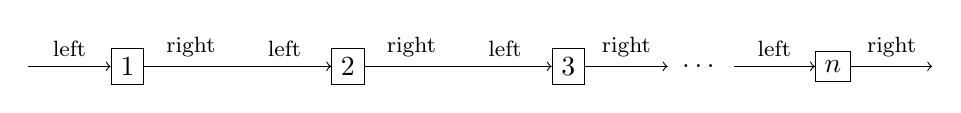
\begin{tikzpicture}[xscale = 2.8]
\draw(0,0) node[draw] (0) {1};
\draw[<-] (0) -- node[above]{\footnotesize\scalastyle left} ++(-0.45,0);
%
\draw(1,0)  node[draw] (1) {2};
\draw[->] (0) -- node[above,near start]{\footnotesize\scalastyle right}
  node[above,near end]{\footnotesize\scalastyle left} (1);
%
\draw(2,0)  node[draw] (2) {3};
\draw[->] (1) -- node[above,near start]{\footnotesize\scalastyle right}
  node[above,near end]{\footnotesize\scalastyle left} (2);
%
\draw[->] (2) -- node[above]{\footnotesize\scalastyle right} ++(0.45,0);
%
\draw(2.6,0) node {\ldots};
%
\draw(3.2,0) node[draw] (n) {$n$};
\draw[<-] (n) -- node[above]{\footnotesize\scalastyle left} ++(-0.45,0);
\draw[->] (n) -- node[above]{\footnotesize\scalastyle right} ++(0.45,0);
\end{tikzpicture}
\end{center}
%
Each component
should receive a stream of values on its \SCALA{left} channel, keep the
largest, and pass the rest to the next process, via its \SCALA{right} channel.
Each process should hold at most two values at any time: the most recently
received value and the largest seen so far.  The end of the input stream
should be signalled by the input channel being closed.  At the end, the sorted
values should be output on the right-most channel.

Implement a testing rig for the sorting network.

Would your network sort more than $n$ input values?

How many messages are sent in total?

How does the execution time depend upon~$n$ (using $O(\_)$ notation).  In
other words, how does the length of the longest totally ordered chain of
messages \( m_1 \prec m_2 \prec \ldots \prec m_k \) depend on~$n$?  Optional:
give an exact value for the length of the longest such chain.
\end{question}

%%%%%

\begin{answer}
%% The question is deliberately vague about how the end of stream should be
%% signalled; the obvious thing to do is to close the channel.
My code is below.  
%
\begin{scala}
import io.threadcso._

/** A process to sort n numbers, using a pipeline. */
class PipeSort(n: Int){
  /** A single node. */
  private def node(left: ?[Int], right: ![Int]) = proc{
    var current = left?()
    repeat{
      val next = left?()
      if(current > next) right!next
      else { right!current; current = next }
    }
    right!current; right.closeOut
  }

  private val chans = Array.fill(n+1)(OneOne[Int])

  /** The input channel to the pipeline. */
  val left = chans(0)

  /** The output channel from the pipeline. */
  val right = chans(n)

  /** The sorting network. */
  def apply(): PROC = || (for(i <- 0 until n) yield node(chans(i), chans(i+1)))
}
\end{scala}

My testing code is below.  The |generator| injects the values from~|xs| into
the network; the |collector| deposits the outputs into~|ys|; at the end we
check that |ys| is a sorted version of~|xs|.  (Note for tutors: there was a
very similar testing framework in lectures, so I suggest just sketching this.)
%
\begin{scala}
import scala.util.Random

/** A testing rig for PipeSort. */
object PipeSortTest{
  /** Send values from xs on right. */
  def generator(right: ![Int], xs: Array[Int]) = proc{
    for(i <- 0 until xs.length) right!xs(i)
    right.closeOut
  }

  /** Receive random numbers on left, and store in ys. */
  def collector(left: ?[Int], ys: Array[Int]) = proc{
    for(i <- 0 until ys.length) ys(i) = left?()
  }

  /** Perform a single test: pass in random numbers; record output; check output
    * is sorted version of input. */
  def doTest = {
    val N = 100
    val xs = Array.fill(N)(Random.nextInt)
    val ys = new Array[Int](N)
    val ps = new PipeSort(N)
    // Run system
    (generator(ps.left, xs) || ps() || collector(ps.right, ys))()
    assert(xs.sorted.sameElements(ys))
  }

  def main(args : Array[String]) = {
    for(i <- 0 until 1000){
      doTest
      if(i%50 == 0) print(".")
    }
    exit
  }
}
\end{scala}

The network would actually sort~$n+1$ values.\footnote{Thanks to Alfonso Bueno
  Orovio for this observation.}  After $n$ inputs, we can get to a state where
every node is holding a value; but no value will be output until either the
input channel is closed, or another value is input; if another value is then
input, it will be treated correctly.

However, the network can't handle more than $n+1$ inputs in general.  Consider
$n+2$ inputs where the final input is the smallest.  The first output will be
the smallest of the first $n+1$ inputs, which is incorrect.


There are $n(n+1)$ messages in total (for $n$ inputs): each of the $n$ values
is passed on each of the $n+1$ channels.

There are $O(n)$ sequentially ordered messages.  The point is that node~$k$
can receive a message concurrently with node~$k+1$ sending a message.  This
means that if node $k$ now holds two values, it can immediately send one to
node~$k+1$.  Thus it  takes about $2n$ rounds for all values to be input.  It
then takes another $O(n)$ rounds (actually about $3n$) for the final value to
propagate along the pipeline.

More precisely, I think there are $5n-3$ sequentially ordered messages:
\begin{itemize}
\item the first node receives $n$ messages and sends $n-1$ messages before
  detecting the input channel is closed; 

\item at this point, the second node holds two values (if $n>2$): it passes
  one on, receives the final value from the first node, passes one value on,
  then detects that its input channel is closed;

\item similarly, there are three communications between each node~$n_k$ 
  detecting its input channel is closed, and the next node $n_{k+1}$ detecting
  its input channel is closed;

\item the final node does a final output. 
\end{itemize}
% 
This gives a total of $(2n-1) + (n-1)\times 3 + 1 = 5n-3$ (for $n>2$).  (I
seem to get a different answer for this every year.)
\end{answer}


% \begin{question}
\begin{enumerate}
\item
Write a definition for a process
\begin{scala}
  def sumStreams(in1: ?[Int], in2: ?[Int], out: ![Int]) = proc{ ... }
\end{scala}
that repeatedly inputs a value from each of its input ports (in either order),
and outputs the sum on the output port.  (Functional programmers might like to
think of this process as implementing \SCALA{zipwith (+)}.)

\item
The Fibonacci numbers \SCALA{fibs} (0, 1, 1, 2, 3, 5, \ldots) can be defined
using the equation
\begin{scala}
  fibs = 0 : sumStreams( fibs, 1:fibs )
\end{scala}
(i.e.\ the stream that starts with 0, and continues with the result of summing
the stream \SCALA{fibs} and the result of pre-pending \SCALA{fibs} with~1). 

Design and implement a circuit with signature
\begin{scala}
  def Fibber(out: ![Int]) = ...
\end{scala}
that outputs the Fibonacci numbers on \SCALA{out}, making use of the above
equation.  Draw a picture to explain your design.  Produce a simple test rig
to test your implementation.
\end{enumerate}
\end{question}

%%%%%

\begin{answer}
We'll produce a system as illustrated below.
\begin{verbatim}
                      fwd
    |---->prefix 0-----------|  
    |                        |
    |                        |
    |                back1   V    out
sum |      prefix 1<-------tee3---->
    |         |              |
    |    back2|              |back3
    |         |              |
    |         V              |
    ----sumStreams<-----------                           
\end{verbatim}
\begin{scala}
import ox.CSO._

object Fibs{

  // Three-way T component
  def tee3[T](in: ?[T], out1: ![T], out2: ![T], out3: ![T]) = proc{
    repeat{
      val v = in?; 
      (proc{ out1!v } || proc{ out2!v } || proc{ out3!v })();
    }
    in.close; out1.close; out2.close; out3.close;
  } 

  // Input values from each input channel, and output their sum
  def sumStreams(in1: ?[Int], in2: ?[Int], out: ![Int]) = proc{
    var x=0; var y=0;
    repeat{
      (proc{ x = in1? } || proc{ y = in2? })();
      out!(x+y); 
    }
    in1.close; in2.close; out.close;
  }

  // From lectures
  def prefix[T](first:T, in: ?[T], out: ![T]) = proc{
    out!first;
    repeat{ out!(in?); };
    in.close; out.close;
  }

  val sum, fwd, back1, back2, back3 = OneOne[Int];

  def Fibber(out: ![Int]) = (
    prefix(0, sum, fwd) || tee3(fwd, out, back1, back3) ||
    prefix(1, back1, back2) || sumStreams(back2, back3, sum)
  );

  // Test rig
  def TestRig = {
    val out = OneOne[Int];
    Fibber(out) || ox.cso.Components.console(out);
  }

  def main(args : Array[String]) = TestRig()
}
\end{scala}
\end{answer}
 Maybe include this

%\begin{nontutequestion}
\Programming
\begin{enumerate}
\item
Write a definition for a component
%
\begin{scala}
def zipwith[L,R,O](f:(L, R)=>O)(lin:?[L], rin:?[R], out:![O]) = proc{ ... }
\end{scala}
%
which repeatedly inputs values \SCALA{l} and \SCALA{r} on \SCALA{lin} and
\SCALA{rin}, respectively, and outputs \SCALA{f(l,r)} on \SCALA{out}. 

\item
An \emph{integrator} is a process with signature
%
\begin{scala}
def integrator(in: ?[Int], out: ![Int]) = ...
\end{scala}
that repeatedly inputs on~\SCALA{in}, and outputs on~\SCALA{out} the sums of
the inputs so far.  That is, if it receives the inputs \SCALA{x1, x2, x3,
  ...}, it outputs \SCALA{x1, x1+x2, x1+x2+x3, ...}.  Design and implement an
integrator as a circuit using \SCALA{zipwith} and other common components.
Draw a diagram to explain your design.  Produce a simple test rig to test the
integrator. 
\end{enumerate}
\end{nontutequestion}

%%%%%

\begin{nontuteanswer} 
\begin{scala}
def zipwith[L,R,O](f:(L, R)=>O)(lin:?[L], rin:?[R], out:![O]) = proc{
  var l = null.asInstanceOf[L]; 
  var r = null.asInstanceOf[R];
  repeat { 
    (proc { l = lin? } || proc { r = rin? })(); 
    out!f(l, r) 
  };   
  lin.close; rin.closein; out.closeout
}
\end{scala}
%
In fact, this is defined as \SCALA{ox.cso.Components.zipwith}.

For the integrator, we'll use a circuit like before (where the first component
is a \SCALA{zipwith} using adition.
%
\begin{verbatim}
                in                       out
 [x,y,z,...] >------>|\    mid     /|-------> [x,x+y,x+y+z,...]
                     |+}--------->{ |
                 +-->|/            \|--+
             addl|                     |back
                 +------<prefix 0<-----+
\end{verbatim}
%
\begin{scala}
import ox.CSO._, ox.cso.Components

object Integrator{

  def integrator(in: ?[Int], out: ![Int]) = {
    val mid, back, addl = OneOne[Int]
    (  Components.zipwith ((x:Int, y:Int)=>x+y) (in, addl, mid)
    || Components.tee (mid, List(out, back))
    || Components.prefix(0)(back, addl)
    )
  }

  // Produce stream of nats
  def nats(out: ![Int]) = proc("nats"){
    var n = 0;
    repeat{ out!n; n+=1; sleep(200) }
  }

  // Test rig, using the above
  def TestRig = {
    val in, out = OneOne[Int];
    ( integrator(in, out) || nats(in) || Components.console(out) )
  }

  def main(args : Array[String]) = TestRig()
}
\end{scala}
The test rig provides the integrator with naturals, and we can check that we
get the triangular numbers out.
\end{nontuteanswer}
 % zipWith and integrator

% \begin{nontutequestion}
In the numerical integration example, we assumed that the number $n$ of
intervals was divisible by the number $ntasks$ of tasks.  How can
we remove this assumption?
\end{nontutequestion}

%%%%%

\begin{nontuteanswer}
The easiest thing to do is to make most tasks of size $\lceil n/ntasks
\rceil$, and to make the last task appropriately smaller.  Making the last
task smaller is likely to make the overall computation finish faster.

It is possible to use a more sophisticated scheme, where all the tasks are of
size $\lceil n/ntasks \rceil$ or $\lfloor n/ntasks \rfloor$, but, frankly,
these don't give any benefits.
\end{nontuteanswer}
 % Remove assumption that \# processors divides \# segments.

\begin{question}
\Programming\ Write a concurrent program to multiply two large $n$ by $n$
matrices~|a| and~|b| together, storing the result in matrix~|c|.  You should
use the bag-of-tasks pattern.  You should consider what a suitable ``task''
should be: remember that making a task too small will mean that workers spend
most of their time waiting to receive the next task.  \textbf{Optional:} carry
out some experiments to assess different sizes of tasks.
% You will probably want to represent each matrix by a two dimensional array.
% Such an array can be initialised in Scala using, e.g.:
% %
% \begin{scala}
% var a = new Array[Array[Int]](N,N);
% \end{scala}
% %
% The element in position $(i,j)$ can be accessed using \SCALA{a(i)(j)}.
\end{question}

%%%%%

\begin{answer}
It makes sense to define a \emph{task} to be the creation of several rows of
the result, say \SCALA{taskSize} rows.  
% The communication overhead is
% $\Theta(n/taskSize)$, so for large arrays, having a task as a single row
% (i.e.\ taking $taskSize=1$) would probably be too small a task (although the
% communication overhead of using a single row would be reasonably small
% compared to the $\Theta(N^3)$ computational cost).  
Taking a task to be a single entry in the result would be too small a task: it
would give a $\Theta(n^2)$ communication overhead.  Using a whole number of
rows (or columns) is easier to program than any other way of splitting up the
problem (e.g.\ into square regions).

There is no need for the workers to return any result to the controller: each
worker can write directly into the result array.  Note that since the tasks
write to disjoint parts of the result array, there are no race conditions. 

Here's my code:
%
\begin{scala}
class Matrix(a: Array[Array[Int]], b: Array[Array[Int]], numWorkers: Int, taskSize: Int){
  private val n = a.size

  /** Array to store the result. */
  private var c = Array.ofDim[Int](n,n)

  /** A task.  The pair (start,end) represents the task of calculating rows [start..end). */
  private type Task = (Int,Int) 

  /** Channel for sending tasks. */
  private val toWorkers = OneMany[Task]

  /** A worker: repeatedly receive tasks, and calculate the relevant rows. */
  private def worker = proc{
    repeat{
      val(start,end) = toWorkers?()
      for(i <- start until end; j <- 0 until n){
	// Calculate value for c(i)(j)
	var sum = 0
	for(k <- 0 until n) sum += a(i)(k)*b(k)(j)
	c(i)(j) = sum
      }
    }
  }

  /** The controller: repeatedly allocate tasks of size taskSize. */
  private def controller = proc{
    var current = 0
    while(current < n){
      toWorkers!(current, current+taskSize min n)
      current += taskSize
    }
    toWorkers.close
  }

  /** calculate the product of a and b. */
  def apply(): Array[Array[Int]] = {
    run(|| (for(w <- 0 until numWorkers) yield worker) || controller)
    c
  }
}
\end{scala}

I ran some informal experiments based around the following function.  The
``warm up'' part is to avoid the effects of JIT compilation.
%
\begin{scala}
  /** Measure times for different task sizes, for matrices of size n and
    * numWorkers worker threads. */
  def timingTest(n: Int, numWorkers: Int) = {
    // # reps; chosen to spend ~3s per task size
    val reps = (300L*Million*numWorkers/(n.toLong*n*n)).toInt
    println("reps = "+reps)
    // Warm up
    for(_ <- 0 until reps){
      val a = randomArray(n); val b = randomArray(n)
      val c = new Matrix(a, b, numWorkers, 2)()
    }
    println("starting")
    for(taskSize <- 1 until 10){
      var elapsed = 0L
      for(_ <- 0 until reps){
        val a = randomArray(n); val b = randomArray(n)
        val start = System.nanoTime
        val c = new Matrix(a, b, numWorkers, taskSize)()
        elapsed += System.nanoTime-start
      }
      println(taskSize+"\t"+elapsed/Million+"ms")
    }
  }
\end{scala}
%
For small values of |n| (around 200) a task size of 2 was often best; with
smaller tasks, the $O(\sm n^2/\sm{taskSize})$ communication overhead meant
that the controller was a bottleneck.  For larger values of |n|, a task size
of~1 was best; each task has $O(\sm n^2)$ computational cost, which is
sufficiently large that the controller is not a bottleneck; and having more
tasks gives better load balancing.  It might be interesting to run experiments
with smaller tasks, say to calculate part of a row of the result.
\end{answer}
 % Matrix multiplication

\begin{nontutequestion}
Suppose you are given two large arrays of |Int|s, |a| and~|b|, neither
of which contains any repetitions.  Describe the design for a
concurrent program to count the number of values that appear in both
arrays.  This problem could be specified (using a couple of functions
from the Scala API) as:
\begin{scala}
  a.count(b.contains(_))
\end{scala}
(You do not need to produce concrete code, unless you want to.)
%%  Briefly explain
%% your design.  
% \textbf{Hint:} use a hash table
% (\url{scala.collection.mutable.HashSet}).  

\end{nontutequestion}

%%%%%

\begin{nontuteanswer}
The easiest way is to split |a| into several segments, one for each worker.
Each worker counts the number of values that appear in both its segment and
in~|b|, and sends the result to a controller.  The controller adds up the
sub-results.  Each worker can calculate its result by putting the elements
of~|b| into a hash table, then counting the number of elements from its
segment that are in the hash table (this avoids quadratic behaviour).  Here's
my code.
%
\begin{scala}
/** Object to count the number of duplicates between a and b, using numWorkers
  * worker threads. */
class CountDups(a: Array[Int], b: Array[Int], numWorkers: Int){
  private val aSize = a.length

  /** Channel for workers to send results to controller. */
  private val toController = ManyOne[Int]

  /** A single worker. */
  private def worker(me: Int) = proc{
    // This worker will deal with a[aStart..aEnd) and all of b
    val aStart = (me*aSize)/numWorkers
    val aEnd = (me+1)*aSize/numWorkers
    // Hash table storing elements of b.
    val bHash = new scala.collection.mutable.HashSet[Int]
    bHash ++= b
    // Iterate through segment of a, counting how many entries are in bHash
    var count = 0
    for(i <- aStart until aEnd; if bHash.contains(a(i))) count += 1 
    // Send result to controller
    toController!count
  }

  /** Variable that ends up holding the result.  While the system is running,
    * only the controller writes to this, and no other thread reads it, so
    * there are no races. */
  private var result = 0

  /** The controller. */
  private def controller = proc{
    for(i <- 0 until numWorkers) result += toController?()
  }

  /** Find the number of duplicates. */
  def apply(): Int = {
    result = 0
    // Run the system
    run(|| (for(i <- 0 until numWorkers) yield worker(i)) || controller)
    result
  }	
}
\end{scala}

An alternative would be to use the bag-of-tasks pattern, where each task
corresponds to a segment of~|a|; note that each worker can re-use its hash
table for multiple tasks. 

There seems no point in splitting \emph{both} |a| and~|b| into multiple
segments, as this wouldn't allow the hash table to be re-used.  

In fact, it is probably sound for the workers to share a single hash table
|bHash| that stores the values from~|b|, as long as all the elements of~|b| are
added to |bHash| before any worker starts.  This assumes that the |contains|
operation for the hash table is thread-safe (i.e.~two threads can safely perform
|contains| concurrently); this will be the case if |contains| performs no
write of a variable (which will often be the case).  It is tempting to arrange
for the workers to share the work of adding the elements of |b| to |bHash|.
However, the |add| operation on the hash table almost certainly isn't
thread-safe; we will see in later chapters how to design a concurrent
datatype, like a hash table, that is thread-safe. 

Testing can be performed by generating random arrays with no repetitions,
running the concurrent algorithm, and then comparing with the result specifed
in the question; this can be repeated many times.
\end{nontuteanswer}


%%% Old version, which doesn't make a lot of sense.

% The obvious approach is to split \SCALA{a} into \SCALA{aSegs} segments, and
% \SCALA{b} into \SCALA{bSegs} segments, and to give a segment of \SCALA{a}
% and a segment of \SCALA{b} to each worker (possibly several pairs of segments,
% but see below).  The worker can count the number of common values in these
% segments by putting the elements of the segment of \SCALA{b}, say, into a hash
% table, and then testing whether each element of the segment of \SCALA{a} is in
% that hash table.  The counts from each worker can be passed to a
% controller,that adds them up. 

% Should we use the bag of tasks pattern, or should each worker deal with a
% single segment of each array?
% A bit of thought shows that taking \SCALA{aSegs*bSegs} greater than the number
% of processes leads to duplicated work: splitting a segment of~\SCALA{a} into
% multiple segments means that the hash table for the segment of~\SCALA{b} has
% to be created extra times; and splitting a segment of~\SCALA{b} into multiple
% segments means that each element of~\SCALA{a} has to be dealt with extra
% times.  We therefore avoid the bag of tasks pattern, and allocate a single
% segment of each array to each worker.  

% Code is not compulsory, but I'll include mine below, anyway.  My experiments
% suggest that this is fastest (on an 8 processor machine) when we take
% \SCALA{aSegs = 1} and \SCALA{bSegs = 8}.  This is an artefact of the relative
% speeds of different operations, and I don't think could have been anticipated
% in advance. 


%% We split \SCALA{a} into \SCALA{aSegs} segments, and \SCALA{b} into
%% \SCALA{bSegs} segments.  Each of the \SCALA{numWorkers = aSegs*bSegs} workers
%% wil work on a segment of \SCALA{a} and a segment of~\SCALA{b}, and count the
%% number of values that appear in both segments, and send the result to the
%% controller.  The elements of the \SCALA{b} segment are put into a hash table
%% to allow fast checking of membership.
%
% \begin{scala}
% // Given arrays a, b, with no repetitions, count the 
% // number of distinct elements in both a and b.

% import ox.CSO._;

% object CountDups{
%   val N = 500000; // size of arrays
%   val a = new Array[Int](N);
%   val b = new Array[Int](N);

%   // Each worker will work on a segment of a and 
%   // a segment of b
%   val aSegs = 1; // number of segments of a
%   val aSegSize = N/aSegs
%   val bSegs = 8; // number of segments of b
%   val bSegSize = N/bSegs
%   val numWorkers = aSegs*bSegs; 

%   // A single worker
%   def Worker(me: Int, toController: ![Int]) = proc{
%     // This worker will deal with a[aStart..aEnd) 
%     // and b[bStart..bEnd) 
%     def aStart = (me/bSegs) * aSegSize;
%     def aEnd = (me/bSegs + 1) * aSegSize;
%     def bStart = (me%bSegs) * bSegSize;
%     def bEnd = (me%bSegs + 1) * bSegSize;

%     // Put all b elements in hash table
%     // val bHash = new java.util.HashSet[Int](bSegSize*2);
%     // for(i <- bStart until bEnd) bHash.add(b(i));
%     val bHash = new scala.collection.mutable.HashSet[Int];
%     for(i <- bStart until bEnd) bHash += b(i);

%     // Now iterate through segment of a, counting how 
%     // many entries are in bHash
%     var count = 0;
%     for(i <- aStart until aEnd)
%       if(bHash.contains(a(i))) count+=1;

%     // Send result to controller
%     toController!count;
%   }

%   // The controller
%   def Controller(toController: ?[Int]){
%     var count = 0;
%     for(i <- 0 until numWorkers) count += (toController?);
%     println(count);
%   }

%   // Initialise arrays
%   def Init{
%     // We set a(i)=i, b(i)=2*i;
%     for(i <- 0 until N){ a(i)=i; b(i)=2*i; }
%   }

%   // Construct system
%   val toController = ManyOne[Int];
%   def Workers =
%     || ( for(i <- 0 until numWorkers) yield 
%            Worker(i, toController) )
%   def System = Controller(toController) || Workers

%   def main(args:Array[String]) = {
%     Init; 
%     val t0 = java.lang.System.currentTimeMillis();
%     System();
%     println("Time taken: "+
%       (java.lang.System.currentTimeMillis()-t0)/1000.0);
%   }
% }
% \end{scala}

% Curiously, the Scala hashtable seems considerably faster than the Java one. 
% \end{nontuteanswer}

% Given two arrays a and b, without repetitions, count the number of distinct
% elements that appear in both a and b. 

%\begin{nontutequestion}
(Optional.)
\begin{enumerate}
\item
Suppose $x$ and $y$ are random numbers, chosen with a uniform distribution on
$[0,1)$.  Show that $Prob(x^2+y^2<1) = \pi/4$.  Hint: use a geometric
  argument.

\item
\Programming\ 
Use this idea to write a concurrent program to estimate the value of $\pi$.

\item
(For those who have taken a course on probability:) Estimate the
  standard deviation of the results given by your program.
\end{enumerate}
\end{nontutequestion}

%%%%%

\begin{nontuteanswer}
For part (a): consider a quarter circle, with centre $(0,0)$, inscribed in the
quadrant $0 \le x,y < 1$.  Then
\begin{eqnarray*}
Prob(x^2+y^2<1) & = & Prob(\mbox{$(x,y)$ is in the quarter circle}) \\
 & = & \mbox{area of quarter circle}/\mbox{area of quadrant} \\
 & = & \pi/4.
\end{eqnarray*}

The program below uses the bag of tasks pattern.  Each task is to generate
\SCALA{taskSize} pairs $(x,y)$ and to count how many satisfy $x^2+y^2<1$.  The
controller compiles the results.
%
\begin{scala}
// Estimate pi, using the fact that if x, y are random 
// numbers in [0,1), then P(x^2+y^2)<1 = pi/4.

import ox.CSO._

object pi{
  val taskSize = 20000;
  val numTasks = 50;
  val numWorkers = 8;

  // val random = new scala.util.Random;

  // The worker receives a signal on toWorkers, generate
  // taskSize random pairs (x,y), and tell controller 
  // (on toController) how many had x^2+y^2 < 1.
  def Worker(toWorkers: ?[Unit], toController: ![Int]) 
  = proc{
    val random = new scala.util.Random;
    repeat{
      toWorkers?;
      var count=0;
      for(i <- 0 until taskSize){
	val x = random.nextDouble; 
        val y = random.nextDouble;
	if(x*x+y*y<1.0) count += 1;
      }
      toController!count;
    }
  }

  def Controller(toWorkers: ![Unit], toController: ?[Int]) 
  = proc{
    // Process to distribute numTasks tasks
    def Sender = proc{
      for(i <- 0 until numTasks) toWorkers!();
      toWorkers.close
    }

    // Process to receive counts and calculate result
    def Receiver = proc{
      var count:Int = 0;
      for(i <- 0 until numTasks) count += (toController?) ;
      println( 
        (4.0*(count:Double)/(taskSize*numTasks)).toString
      );
    }

    (Sender || Receiver)();
  }

  // Construct system
  val toWorkers = OneMany[Unit];
  val toController = ManyOne[Int];
  
  def Workers = 
    || ( for(i <- 0 until numWorkers) yield
           Worker(toWorkers, toController) );

  def System = 
    Controller(toWorkers, toController) || Workers

  def main(args:Array[String]) = {
    val t0 = java.lang.System.currentTimeMillis();
    System();
    println("Time taken: "+
      (java.lang.System.currentTimeMillis()-t0)/1000.0);
  }
}
\end{scala}

Each worker can be given their own random number generator, or they can share
a single one.  In my tests, the latter is about 20 times slower, which is quite
surprising.  I suspect the reason it is more than \SCALA{numWorkers} times
slower is that the state of the random number generator has to be copied to
the appropriate cache for each random number.

If we let $n$ be the number of samples, then the number of samples that
satisfy the property $x^2+y^2<1$ has binomial distribution $Binom(n,\pi/4)$,
which has variance $n.\pi/4.(1-\pi/4)$, standard deviation
$\sqrt(n.\pi/4.(1-\pi/4))$, and so a standard deviation on the final result of
$4.\sqrt(\pi/4.(1-\pi/4)) / \sqrt n \approx 1.64 / \sqrt n$.  For $n = 10^6$, as
above, this is about $0.00164$.  This is consistent with the experimental
observation that the program is normally accurate to about two decimal places.
\end{nontuteanswer}



%% \resetquestionnumbers
%% \nontuteanswersonly
%% \begin{nontutequestion}
Consider a web browser that supports multiple tabs (i.e.~different
tabs for different web pages).  Why might it be beneficial to use
concurrency in the implementation of such a web browser?  Would this
still make sense on a uni-processor computer?  What problems might
arise from such a design?
\end{nontutequestion}

%%%%%

\begin{nontuteanswer}
There are two main reasons: ease of implementation, and efficiency.

Building a web browser this way is easier!  The different tabs are largely
independent.  It's far easier to write a thread that deals with a single tab,
and run $n$ such threads, than to write a single thread that deals with all
$n$ tabs.  Each tab thread will probably need to interact with some main
browser thread, but that's relatively straightforward.

In terms of efficiency, concurrency might be used to give better response to
user actions (i.e.\ lower latency), and better overall performance (i.e.\
higher throughput); of these, the former seems more important.

As an example of why a sequential implementation might be unsatisfactory,
consider a user who has two tabs open, one viewing a page that automatically
re-loads every few minutes, and another that the user is actively reading.
Suppose the user tries to scroll down in the second page just after the first
page starts a re-load; then the user has to wait until the re-load completes
before the second page scrolls; this could take several seconds, and so annoy
the user.  (The Firefox browser used to act in this way.)  If the different
tabs used different processes, then they could run concurrently so the user
wouldn't see this delay.  This would still be the case on a uni-processor
machine: the fact that the two processes are competing for the processor would
slow things down a bit, but probably not enough for the user to notice.

The problem is, of course, that two processes might try to access some shared
data (e.g.~the history list) simultaneously, leading to race conditions.
These race conditions can be avoided by careful programming: see the rest of
the course!
\end{nontuteanswer}
 % Why make a web browser use concurrency?  

%\begin{nontutequestion}
Suppose process \SCALA{P} performs $m$ atomic actions (sequentially), and
process \SCALA{Q} performs $n$ atomic actions (sequentially).  When \SCALA{P}
and \SCALA{Q} are run in parallel, how many interleavings of atomic actions
are there?
\end{nontutequestion}
%
\begin{nontuteanswer}
There are a total of $m+n$ atomic actions.  The number of ways of choosing
which $m$ of these belong to~\SCALA{P} is
\[
\left( \begin{array}{@{}c@{}} m+n \\ m \end{array} \right) =
\frac{(m+n)!}{m! n!}
\]
\end{nontuteanswer}

 % Count number of execution seqs - formula

%\begin{question}
Consider the code below.
%
\begin{scala}
var x = 0

def p = proc{ x = x+1; x = x+2 }

def q = proc{ x = x+4 }

def system = p || q
\end{scala}
%
Suppose the atomic actions are reading or writing a variable.
When \SCALA{system} is run, what are the possible final values of \SCALA{x}?
Draw a diagram to illustrate the different possible execution paths.
\end{question}
%
\begin{answer}
The diagram below shows all interleavings until one process terminates, at
which point the system becomes deterministic.  Each label is a triple: the
process doing the event ($P$ or $Q$); an indication of the action (``r'' for
read or ``w'' for write); and the value read or written.  The figures in
circles then show the final value of \SCALA{x} that will result.  The possible
values are 3, 4, 5, 6, 7.  As a check, the diagram shows 
\( {\scriptstyle
  \left( \begin{array}{@{}c@{}} \scriptstyle 6 \\[-1mm] \scriptstyle
    4 \end{array} \right)} = 15 \) interleavings.
%
\begin{center}
\ 
\includegraphics[width=12cm]{interleavings2.eps}\ 
\end{center}
%
The point is that even a very simple program with dependent atomic actions can
become very difficult to understand. 
\end{answer}
 % based on Andrews 2.10; results of particular
                       % interleaving 

%% based on Andrews 2.15
\begin{question}
Consider the code below.
%
\begin{scala}
var x = 0; var y = 10

def p = proc{ while(x != y) x = x+1 }

def q = proc{ while(x != y) y = y-1 }

def system = p || q
\end{scala}
%
Will the process \SCALA{system} terminate?  Explain your answer.
\end{question}
%
\begin{answer}
It might or might not terminate.

Consider an execution where we reach a state with \SCALA{x=4} and \SCALA{y=5},
both processes evaluate \SCALA{x!=y} in this state and enter the body of the
loop.  Now suppose each loop body is executed, giving \SCALA{x=5} and
\SCALA{y=4}.  Subsequently we always have \SCALA{x>y}, so neither process
terminates.

Alternatively, again suppose we reach a state with \SCALA{x=4} and
\SCALA{y=5}, both processes evaluate \SCALA{x!=y} in this state and enter the
body of the loop.  Now suppose \SCALA{p} runs, setting \SCALA{x=5}, evaluates
the guard which is now true, and terminates.  However, when \SCALA{q} runs, it
sets \SCALA{y=4}, so never terminates.  Similarly, it is possible
for~\SCALA{q} to terminate, but not~\SCALA{p}.

There are also problems that are caused by the use of caching.  For example,
|p| could reach a state with |x = 6|, while working with |y = 10| in its
cache; and |q| could reach a state with |y = 4|, while working with |x = 0| in
cache.  When they do refresh their caches, they will again run forever.  


It is easy to find executions where both terminate.
\end{answer}
 % based on Andrews 2.15

{\setnontutequestion\begin{question}
Consider an object representing a bank account, from the following class.
%
\begin{scala}
class Account{
  private var balance = 0

  def credit(value: Int) = atomically{ balance += value }

  def canDebit(value: Int): Boolean = atomically{ balance >= value }

  def debit(value: Int) = atomically{ balance -= value }
}
\end{scala}
%
The ``|atomically|'' pseudocode is intended to indicate that each
procedure is performed atomically (we will see how to do this in a
later chapter).

A process that wants to perform a debit should first of all call
\SCALA{canDebit}, to avoid the account from going overdrawn; for example
%
\begin{scala}[showstringspaces=false]
  if(account.canDebit(value)) account.debit(value)
  else println("Debit not allowed!")
\end{scala}

What can go wrong if two processes execute the above code at the same
time?  Sketch a solution to this problem.
\end{question}

%%%%%

\begin{answer}
Suppose the current balance is 100, and both processes want to debit 100;
clearly only one should succeed.  Both processes could call
\SCALA{canDebit(value)}, getting back the result \SCALA{true}.  They would
then both call \SCALA{debit}, leading to the account balance becoming $-$100.
This is a time-of-check to time-of-use (TOCTTOU) problem: the check that there
is enough money in the account is no longer valid when the debit is
performed. 

The point is that the \SCALA{canDebit} action of one process and the
\SCALA{debit} action of the other are not independent.  This leads to a race
condition.

The obvious way to avoid this problem is to combine the \SCALA{canDebit} and
\SCALA{debit} actions into a single atomic action within the \SCALA{Account}
class.  Something like
%
\begin{scala}
/** Attempt to debit value.  Return true if successful. */
def tryDebit(value: Int): Boolean = atomically{
  if(balance >= value){ balance -= value; true } else false
}
\end{scala}
% 
The calling code (outside the |Account| class) can do the right thing with the
boolean result. 
\end{answer}

} % Account with race condition.

\begin{question}
\begin{figure}
\begin{scala}
class Queue[A]{
  /** A node in the linked list. */
  private class Node(val datum: A, var next: Node)

  /** The dummy header node. */
  private var head = new Node(null.asInstanceOf[A], null)

  /** The last node in the list. */
  private var last = head

  /** Is the queue empty? */
  def isEmpty = last == head

  /** Add x to the queue. */
  def enqueue(x: A) = {
    val node = new Node(x, null); last.next = node; last = node
  }

  /** Dequeue a value.  Pre: the queue is not empty. */
  def dequeue: A = {
    require(!isEmpty); head = head.next; head.datum
  }
}
\end{scala}
\caption{A sequential queue based on a linked list.}
\label{fig:queue}
\end{figure}

Figure~\ref{fig:queue} gives the implementation of a queue based on a linked
list.  The implementation is correct when the queue is used sequentially.
However, if the queue is used concurrently (i.e.~with two or more threads
calling the operations concurrently), then it can go wrong in a number of
different ways.  
%
%I have spotted six essentially different ways in which it can go wrong.
Describe as many as possible essentially different ways in which it can go
wrong (I have spotted six essentially different ways).
%
For the purposes of this question, you should ignore problems caused by
caching or compiler optimisations (those introduce many more ways in which the
implementation can go wrong).
\end{question}

%%%%%%%%%%%%%%%%%%%%%%%%%%%%%%%%%%%%%%%%%%%%%%%%%%%%%%%

\begin{answer}
A thoughtful student might ask ``What does correct mean, here?''  The property
we would like is that the operation invocations appear to take place in a
one-at-a-time order (so without interfering with one another), in an order
compatible with the temporal order of the invocations (so if one invocation
returns before the other is called, they should have an effect in that order),
and giving results as one would expect for a sequential execution.  This
property is called \emph{linearization}: we'll see it later in the course.  It
fits with programmers' mental models. 

Here are some problems I spotted.  I'm sure there are others.
%%   In these examples, I will assume that there are no issues concerning
%% caches or compiler optimisations: such issues will introduce many more ways
%% of things going wrong.  %
\begin{enumerate}
\item
The signature isn't really suitable for a concurrent datatype.  Consider code
like the following, to check the precondition of the |dequeue| operation:
%
\begin{scala}
  if(!queue.isEmpty){ val x = queue.dequeue; ... }
\end{scala}
%
A thread~$t$ could check that the queue is non-empty; then other threads could
perform |dequeue|s so as to empty the queue; then when $t$ calls |dequeue|,
the |require| check will fail.  Better would be to have a signature such as
\begin{scala}
  def dequeue: Option[A] = ...
\end{scala}
that returns |None| when the queue is empty, or |Some(x)| if |x| is dequeued.

%%%%%

\item (Somewhat similar to the previous item.)  A thread~$t$ could call
  |dequeue| when the queue is non-empty, so the |require| passes.  But then
  other threads could perform dequeues, to leave the queue empty (so
  \SCALA{head.next = null}).  When $t$ continues, it sets |head| to null, and
  the expression |head.datum| gives a null-pointer exception.

%%%%%

\item Suppose threads~$t_1$ and~$t_2$ call |enqueue| concurrently, enqueueing
  $x_1$ and~$x_2$, respectively.  Each creates a new node, $n_1$ and~$n_2$.
  Then if $t_1$ and~$t_2$ each updates |last.next| to point to their node, in
  that order, the latter will overwrite the former, so $n_1$ isn't connected
  to the list (so the~$x_1$ is lost).  Further, if $t_2$ then updates |last|
  before~$t_1$, then it will end up pointing to~$n_1$, so |last| will no
  longer be reachable from |head|; this means that the results of all
  subsequent enqueues will be lost.

%%%%%

\item Now suppose threads~$t_1$ and~$t_2$ call |dequeue| concurrently, and
  each reads |head| obtaining the same node~$n$.  Then both will set |head| to
  $n$|.next|, and both will return $n$|.datum|: the same value is dequeued
  twice.

%%%%%

\item Suppose thread $t_1$ calls |dequeue|, and advances |head| to node~$n_1$,
  but stalls before reading |head.datum|.  Suppose now thread~$t_2$ calls
  dequeue, advances |head| to $n_2 = n_1$|.next|, and returns $n_2$|.datum|.
  Then thread~$t_1$ can resume, read |head = |$n_2$, and
  return $n_2$|.datum|.  This value has been returned twice, but the value
  in~$n_1$ was lost. 

\item Suppose thread $t_1$ calls |isEmpty| when the list contains two nodes,
  $n_1 = \sm{head}$ and $n_2 = \sm{last}$ with $n_1.\sm{next} = n_2$; and
  suppose it reads $\sm{last} = n_2$ and stalls.  Suppose then thread~$t_2$
  enqueues another value; and then thread~$t_3$ dequeues a value, setting
  $\sm{head} = n_2$.  Then $t_1$ can resume and read $\sm{head} = n_2$; it
  returns |true| even though the queue was non-empty throughout the
  invocation. 
%
  Changing the definition to
  \begin{scala}
  def isEmpty = head == last
  \end{scala}%
  avoids this problem (assuming no compiler optimisations, etc.).
\end{enumerate}

A solution (to the last five issues) is to adapt the implementation so that
each invocation runs in isolation.  This is the approach we'll adopt later in
the course.  
\end{answer}
 % queue based on linked list, with races

%\begin{question}
\Programming\
Write a definition for a process
%
\begin{scala}
def Merge(left: ?[Int], right: ?[Int], out: ![Int]) = proc ...
\end{scala}
%
that inputs two ascending non-empty streams of integers on \SCALA{left} and
\SCALA{right}, merges them into a single ascending stream, and outputs that on
\SCALA{out}.  The process should hold at most one value at a time from each of
the input streams.  You may assume that the input streams are never closed.
% You may not use \SCALA{ox.cso.Components.merge}.
\end{question}
%
\begin{answer}
%% When one of the input channels is closed, causing the program to break out of
%% the \SCALA{repeat} loop below, we need to know whether the values of \SCALA{l}
%% and \SCALA{r} have already been output; we use the flag \SCALA{invalid} for
%% this.
%
\begin{scala}
import ox.CSO._
import ox.cso.Components._

object MergeStreams{
  // Merge two non-empty ascending streams
  def Merge(left: ?[Int], right: ?[Int], out: ![Int]) 
  = proc("Merge"){
    // Invariant: l is last value read from left; 
    // r is last value read from right
    var l = left?; var r = right?;
    repeat{
      if(l<=r){ out!l; l=left? }
      else{ out!r; r=right? }
    }
    left.close; right.close; out.close;
  }

  val random = new scala.util.Random ;

  // Produce an ascending stream of n Ints on out
  def Producer(n:Int, out: ![Int]) = proc("Producer"){
    var current = 0;
    for(i <- 0 until n){ 
      current += random.nextInt(5); 
      println("producing "+current); 
      out!current;
    }
    out.close
  }

  val left = OneOne[Int]; 
  val right = OneOne[Int];
  val out = OneOne[Int];

  def System(n:Int) = (
    Merge(left, right, out) || Producer(n, left) 
    || Producer(n, right) || console(out) 
  )

  def main(args : Array[String]) = 
    System( 
      if(args.length>0)
        Integer.valueOf(args(0)).intValue()
      else 10 
    )();
}
\end{scala}
%
[Students should provide some sensible test results.]
\end{answer}
 % merge two ordered streams

%\begin{question}
CSO channels are rather like CSP events.  Describe one or two ways in
which they are different.
\end{question}

%%%%%

\begin{answer}
CSP processes are defined in terms of events, and so CSP does not distinguish
between input and output (although there are constructs that behave like input
and output); however, channels in CSO are uni-directional, and so input and
output are distinguished.  This means that if a CSO process is willing to
input from a channel, it should be willing to input an arbitrary value; there
is no equivalent of the CSP selective input, e.g. $in?x:A \then \ldots$.

Also, CSO communications are always synchronisations between exactly two
processes, whereas in CSP any number of processes can synchronise on an
event. 
\end{answer}
 % Compare CSP events and CSO communications.

% Based on Andrews Ex 7.3
\begin{question}
\Programming\ Implement a program to sort $n$ integers using a pipeline of $n$
components, as depicted below (note that the value of $n$ is known in
advance).
%
\begin{center}
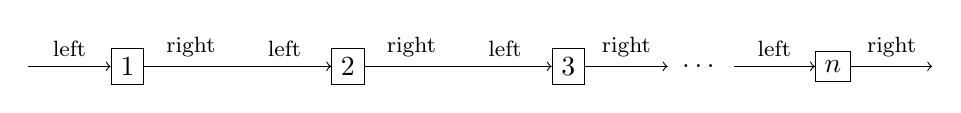
\begin{tikzpicture}[xscale = 2.8]
\draw(0,0) node[draw] (0) {1};
\draw[<-] (0) -- node[above]{\footnotesize\scalastyle left} ++(-0.45,0);
%
\draw(1,0)  node[draw] (1) {2};
\draw[->] (0) -- node[above,near start]{\footnotesize\scalastyle right}
  node[above,near end]{\footnotesize\scalastyle left} (1);
%
\draw(2,0)  node[draw] (2) {3};
\draw[->] (1) -- node[above,near start]{\footnotesize\scalastyle right}
  node[above,near end]{\footnotesize\scalastyle left} (2);
%
\draw[->] (2) -- node[above]{\footnotesize\scalastyle right} ++(0.45,0);
%
\draw(2.6,0) node {\ldots};
%
\draw(3.2,0) node[draw] (n) {$n$};
\draw[<-] (n) -- node[above]{\footnotesize\scalastyle left} ++(-0.45,0);
\draw[->] (n) -- node[above]{\footnotesize\scalastyle right} ++(0.45,0);
\end{tikzpicture}
\end{center}
%
Each component
should receive a stream of values on its \SCALA{left} channel, keep the
largest, and pass the rest to the next process, via its \SCALA{right} channel.
Each process should hold at most two values at any time: the most recently
received value and the largest seen so far.  The end of the input stream
should be signalled by the input channel being closed.  At the end, the sorted
values should be output on the right-most channel.

Implement a testing rig for the sorting network.

Would your network sort more than $n$ input values?

How many messages are sent in total?

How does the execution time depend upon~$n$ (using $O(\_)$ notation).  In
other words, how does the length of the longest totally ordered chain of
messages \( m_1 \prec m_2 \prec \ldots \prec m_k \) depend on~$n$?  Optional:
give an exact value for the length of the longest such chain.
\end{question}

%%%%%

\begin{answer}
%% The question is deliberately vague about how the end of stream should be
%% signalled; the obvious thing to do is to close the channel.
My code is below.  
%
\begin{scala}
import io.threadcso._

/** A process to sort n numbers, using a pipeline. */
class PipeSort(n: Int){
  /** A single node. */
  private def node(left: ?[Int], right: ![Int]) = proc{
    var current = left?()
    repeat{
      val next = left?()
      if(current > next) right!next
      else { right!current; current = next }
    }
    right!current; right.closeOut
  }

  private val chans = Array.fill(n+1)(OneOne[Int])

  /** The input channel to the pipeline. */
  val left = chans(0)

  /** The output channel from the pipeline. */
  val right = chans(n)

  /** The sorting network. */
  def apply(): PROC = || (for(i <- 0 until n) yield node(chans(i), chans(i+1)))
}
\end{scala}

My testing code is below.  The |generator| injects the values from~|xs| into
the network; the |collector| deposits the outputs into~|ys|; at the end we
check that |ys| is a sorted version of~|xs|.  (Note for tutors: there was a
very similar testing framework in lectures, so I suggest just sketching this.)
%
\begin{scala}
import scala.util.Random

/** A testing rig for PipeSort. */
object PipeSortTest{
  /** Send values from xs on right. */
  def generator(right: ![Int], xs: Array[Int]) = proc{
    for(i <- 0 until xs.length) right!xs(i)
    right.closeOut
  }

  /** Receive random numbers on left, and store in ys. */
  def collector(left: ?[Int], ys: Array[Int]) = proc{
    for(i <- 0 until ys.length) ys(i) = left?()
  }

  /** Perform a single test: pass in random numbers; record output; check output
    * is sorted version of input. */
  def doTest = {
    val N = 100
    val xs = Array.fill(N)(Random.nextInt)
    val ys = new Array[Int](N)
    val ps = new PipeSort(N)
    // Run system
    (generator(ps.left, xs) || ps() || collector(ps.right, ys))()
    assert(xs.sorted.sameElements(ys))
  }

  def main(args : Array[String]) = {
    for(i <- 0 until 1000){
      doTest
      if(i%50 == 0) print(".")
    }
    exit
  }
}
\end{scala}

The network would actually sort~$n+1$ values.\footnote{Thanks to Alfonso Bueno
  Orovio for this observation.}  After $n$ inputs, we can get to a state where
every node is holding a value; but no value will be output until either the
input channel is closed, or another value is input; if another value is then
input, it will be treated correctly.

However, the network can't handle more than $n+1$ inputs in general.  Consider
$n+2$ inputs where the final input is the smallest.  The first output will be
the smallest of the first $n+1$ inputs, which is incorrect.


There are $n(n+1)$ messages in total (for $n$ inputs): each of the $n$ values
is passed on each of the $n+1$ channels.

There are $O(n)$ sequentially ordered messages.  The point is that node~$k$
can receive a message concurrently with node~$k+1$ sending a message.  This
means that if node $k$ now holds two values, it can immediately send one to
node~$k+1$.  Thus it  takes about $2n$ rounds for all values to be input.  It
then takes another $O(n)$ rounds (actually about $3n$) for the final value to
propagate along the pipeline.

More precisely, I think there are $5n-3$ sequentially ordered messages:
\begin{itemize}
\item the first node receives $n$ messages and sends $n-1$ messages before
  detecting the input channel is closed; 

\item at this point, the second node holds two values (if $n>2$): it passes
  one on, receives the final value from the first node, passes one value on,
  then detects that its input channel is closed;

\item similarly, there are three communications between each node~$n_k$ 
  detecting its input channel is closed, and the next node $n_{k+1}$ detecting
  its input channel is closed;

\item the final node does a final output. 
\end{itemize}
% 
This gives a total of $(2n-1) + (n-1)\times 3 + 1 = 5n-3$ (for $n>2$).  (I
seem to get a different answer for this every year.)
\end{answer}


% \begin{question}
\begin{enumerate}
\item
Write a definition for a process
\begin{scala}
  def sumStreams(in1: ?[Int], in2: ?[Int], out: ![Int]) = proc{ ... }
\end{scala}
that repeatedly inputs a value from each of its input ports (in either order),
and outputs the sum on the output port.  (Functional programmers might like to
think of this process as implementing \SCALA{zipwith (+)}.)

\item
The Fibonacci numbers \SCALA{fibs} (0, 1, 1, 2, 3, 5, \ldots) can be defined
using the equation
\begin{scala}
  fibs = 0 : sumStreams( fibs, 1:fibs )
\end{scala}
(i.e.\ the stream that starts with 0, and continues with the result of summing
the stream \SCALA{fibs} and the result of pre-pending \SCALA{fibs} with~1). 

Design and implement a circuit with signature
\begin{scala}
  def Fibber(out: ![Int]) = ...
\end{scala}
that outputs the Fibonacci numbers on \SCALA{out}, making use of the above
equation.  Draw a picture to explain your design.  Produce a simple test rig
to test your implementation.
\end{enumerate}
\end{question}

%%%%%

\begin{answer}
We'll produce a system as illustrated below.
\begin{verbatim}
                      fwd
    |---->prefix 0-----------|  
    |                        |
    |                        |
    |                back1   V    out
sum |      prefix 1<-------tee3---->
    |         |              |
    |    back2|              |back3
    |         |              |
    |         V              |
    ----sumStreams<-----------                           
\end{verbatim}
\begin{scala}
import ox.CSO._

object Fibs{

  // Three-way T component
  def tee3[T](in: ?[T], out1: ![T], out2: ![T], out3: ![T]) = proc{
    repeat{
      val v = in?; 
      (proc{ out1!v } || proc{ out2!v } || proc{ out3!v })();
    }
    in.close; out1.close; out2.close; out3.close;
  } 

  // Input values from each input channel, and output their sum
  def sumStreams(in1: ?[Int], in2: ?[Int], out: ![Int]) = proc{
    var x=0; var y=0;
    repeat{
      (proc{ x = in1? } || proc{ y = in2? })();
      out!(x+y); 
    }
    in1.close; in2.close; out.close;
  }

  // From lectures
  def prefix[T](first:T, in: ?[T], out: ![T]) = proc{
    out!first;
    repeat{ out!(in?); };
    in.close; out.close;
  }

  val sum, fwd, back1, back2, back3 = OneOne[Int];

  def Fibber(out: ![Int]) = (
    prefix(0, sum, fwd) || tee3(fwd, out, back1, back3) ||
    prefix(1, back1, back2) || sumStreams(back2, back3, sum)
  );

  // Test rig
  def TestRig = {
    val out = OneOne[Int];
    Fibber(out) || ox.cso.Components.console(out);
  }

  def main(args : Array[String]) = TestRig()
}
\end{scala}
\end{answer}
 Maybe include this

%\begin{nontutequestion}
\Programming
\begin{enumerate}
\item
Write a definition for a component
%
\begin{scala}
def zipwith[L,R,O](f:(L, R)=>O)(lin:?[L], rin:?[R], out:![O]) = proc{ ... }
\end{scala}
%
which repeatedly inputs values \SCALA{l} and \SCALA{r} on \SCALA{lin} and
\SCALA{rin}, respectively, and outputs \SCALA{f(l,r)} on \SCALA{out}. 

\item
An \emph{integrator} is a process with signature
%
\begin{scala}
def integrator(in: ?[Int], out: ![Int]) = ...
\end{scala}
that repeatedly inputs on~\SCALA{in}, and outputs on~\SCALA{out} the sums of
the inputs so far.  That is, if it receives the inputs \SCALA{x1, x2, x3,
  ...}, it outputs \SCALA{x1, x1+x2, x1+x2+x3, ...}.  Design and implement an
integrator as a circuit using \SCALA{zipwith} and other common components.
Draw a diagram to explain your design.  Produce a simple test rig to test the
integrator. 
\end{enumerate}
\end{nontutequestion}

%%%%%

\begin{nontuteanswer} 
\begin{scala}
def zipwith[L,R,O](f:(L, R)=>O)(lin:?[L], rin:?[R], out:![O]) = proc{
  var l = null.asInstanceOf[L]; 
  var r = null.asInstanceOf[R];
  repeat { 
    (proc { l = lin? } || proc { r = rin? })(); 
    out!f(l, r) 
  };   
  lin.close; rin.closein; out.closeout
}
\end{scala}
%
In fact, this is defined as \SCALA{ox.cso.Components.zipwith}.

For the integrator, we'll use a circuit like before (where the first component
is a \SCALA{zipwith} using adition.
%
\begin{verbatim}
                in                       out
 [x,y,z,...] >------>|\    mid     /|-------> [x,x+y,x+y+z,...]
                     |+}--------->{ |
                 +-->|/            \|--+
             addl|                     |back
                 +------<prefix 0<-----+
\end{verbatim}
%
\begin{scala}
import ox.CSO._, ox.cso.Components

object Integrator{

  def integrator(in: ?[Int], out: ![Int]) = {
    val mid, back, addl = OneOne[Int]
    (  Components.zipwith ((x:Int, y:Int)=>x+y) (in, addl, mid)
    || Components.tee (mid, List(out, back))
    || Components.prefix(0)(back, addl)
    )
  }

  // Produce stream of nats
  def nats(out: ![Int]) = proc("nats"){
    var n = 0;
    repeat{ out!n; n+=1; sleep(200) }
  }

  // Test rig, using the above
  def TestRig = {
    val in, out = OneOne[Int];
    ( integrator(in, out) || nats(in) || Components.console(out) )
  }

  def main(args : Array[String]) = TestRig()
}
\end{scala}
The test rig provides the integrator with naturals, and we can check that we
get the triangular numbers out.
\end{nontuteanswer}
 % zipWith and integrator

% \begin{nontutequestion}
In the numerical integration example, we assumed that the number $n$ of
intervals was divisible by the number $ntasks$ of tasks.  How can
we remove this assumption?
\end{nontutequestion}

%%%%%

\begin{nontuteanswer}
The easiest thing to do is to make most tasks of size $\lceil n/ntasks
\rceil$, and to make the last task appropriately smaller.  Making the last
task smaller is likely to make the overall computation finish faster.

It is possible to use a more sophisticated scheme, where all the tasks are of
size $\lceil n/ntasks \rceil$ or $\lfloor n/ntasks \rfloor$, but, frankly,
these don't give any benefits.
\end{nontuteanswer}
 % Remove assumption that \# processors divides \# segments.

\begin{question}
\Programming\ Write a concurrent program to multiply two large $n$ by $n$
matrices~|a| and~|b| together, storing the result in matrix~|c|.  You should
use the bag-of-tasks pattern.  You should consider what a suitable ``task''
should be: remember that making a task too small will mean that workers spend
most of their time waiting to receive the next task.  \textbf{Optional:} carry
out some experiments to assess different sizes of tasks.
% You will probably want to represent each matrix by a two dimensional array.
% Such an array can be initialised in Scala using, e.g.:
% %
% \begin{scala}
% var a = new Array[Array[Int]](N,N);
% \end{scala}
% %
% The element in position $(i,j)$ can be accessed using \SCALA{a(i)(j)}.
\end{question}

%%%%%

\begin{answer}
It makes sense to define a \emph{task} to be the creation of several rows of
the result, say \SCALA{taskSize} rows.  
% The communication overhead is
% $\Theta(n/taskSize)$, so for large arrays, having a task as a single row
% (i.e.\ taking $taskSize=1$) would probably be too small a task (although the
% communication overhead of using a single row would be reasonably small
% compared to the $\Theta(N^3)$ computational cost).  
Taking a task to be a single entry in the result would be too small a task: it
would give a $\Theta(n^2)$ communication overhead.  Using a whole number of
rows (or columns) is easier to program than any other way of splitting up the
problem (e.g.\ into square regions).

There is no need for the workers to return any result to the controller: each
worker can write directly into the result array.  Note that since the tasks
write to disjoint parts of the result array, there are no race conditions. 

Here's my code:
%
\begin{scala}
class Matrix(a: Array[Array[Int]], b: Array[Array[Int]], numWorkers: Int, taskSize: Int){
  private val n = a.size

  /** Array to store the result. */
  private var c = Array.ofDim[Int](n,n)

  /** A task.  The pair (start,end) represents the task of calculating rows [start..end). */
  private type Task = (Int,Int) 

  /** Channel for sending tasks. */
  private val toWorkers = OneMany[Task]

  /** A worker: repeatedly receive tasks, and calculate the relevant rows. */
  private def worker = proc{
    repeat{
      val(start,end) = toWorkers?()
      for(i <- start until end; j <- 0 until n){
	// Calculate value for c(i)(j)
	var sum = 0
	for(k <- 0 until n) sum += a(i)(k)*b(k)(j)
	c(i)(j) = sum
      }
    }
  }

  /** The controller: repeatedly allocate tasks of size taskSize. */
  private def controller = proc{
    var current = 0
    while(current < n){
      toWorkers!(current, current+taskSize min n)
      current += taskSize
    }
    toWorkers.close
  }

  /** calculate the product of a and b. */
  def apply(): Array[Array[Int]] = {
    run(|| (for(w <- 0 until numWorkers) yield worker) || controller)
    c
  }
}
\end{scala}

I ran some informal experiments based around the following function.  The
``warm up'' part is to avoid the effects of JIT compilation.
%
\begin{scala}
  /** Measure times for different task sizes, for matrices of size n and
    * numWorkers worker threads. */
  def timingTest(n: Int, numWorkers: Int) = {
    // # reps; chosen to spend ~3s per task size
    val reps = (300L*Million*numWorkers/(n.toLong*n*n)).toInt
    println("reps = "+reps)
    // Warm up
    for(_ <- 0 until reps){
      val a = randomArray(n); val b = randomArray(n)
      val c = new Matrix(a, b, numWorkers, 2)()
    }
    println("starting")
    for(taskSize <- 1 until 10){
      var elapsed = 0L
      for(_ <- 0 until reps){
        val a = randomArray(n); val b = randomArray(n)
        val start = System.nanoTime
        val c = new Matrix(a, b, numWorkers, taskSize)()
        elapsed += System.nanoTime-start
      }
      println(taskSize+"\t"+elapsed/Million+"ms")
    }
  }
\end{scala}
%
For small values of |n| (around 200) a task size of 2 was often best; with
smaller tasks, the $O(\sm n^2/\sm{taskSize})$ communication overhead meant
that the controller was a bottleneck.  For larger values of |n|, a task size
of~1 was best; each task has $O(\sm n^2)$ computational cost, which is
sufficiently large that the controller is not a bottleneck; and having more
tasks gives better load balancing.  It might be interesting to run experiments
with smaller tasks, say to calculate part of a row of the result.
\end{answer}
 % Matrix multiplication

\begin{nontutequestion}
Suppose you are given two large arrays of |Int|s, |a| and~|b|, neither
of which contains any repetitions.  Describe the design for a
concurrent program to count the number of values that appear in both
arrays.  This problem could be specified (using a couple of functions
from the Scala API) as:
\begin{scala}
  a.count(b.contains(_))
\end{scala}
(You do not need to produce concrete code, unless you want to.)
%%  Briefly explain
%% your design.  
% \textbf{Hint:} use a hash table
% (\url{scala.collection.mutable.HashSet}).  

\end{nontutequestion}

%%%%%

\begin{nontuteanswer}
The easiest way is to split |a| into several segments, one for each worker.
Each worker counts the number of values that appear in both its segment and
in~|b|, and sends the result to a controller.  The controller adds up the
sub-results.  Each worker can calculate its result by putting the elements
of~|b| into a hash table, then counting the number of elements from its
segment that are in the hash table (this avoids quadratic behaviour).  Here's
my code.
%
\begin{scala}
/** Object to count the number of duplicates between a and b, using numWorkers
  * worker threads. */
class CountDups(a: Array[Int], b: Array[Int], numWorkers: Int){
  private val aSize = a.length

  /** Channel for workers to send results to controller. */
  private val toController = ManyOne[Int]

  /** A single worker. */
  private def worker(me: Int) = proc{
    // This worker will deal with a[aStart..aEnd) and all of b
    val aStart = (me*aSize)/numWorkers
    val aEnd = (me+1)*aSize/numWorkers
    // Hash table storing elements of b.
    val bHash = new scala.collection.mutable.HashSet[Int]
    bHash ++= b
    // Iterate through segment of a, counting how many entries are in bHash
    var count = 0
    for(i <- aStart until aEnd; if bHash.contains(a(i))) count += 1 
    // Send result to controller
    toController!count
  }

  /** Variable that ends up holding the result.  While the system is running,
    * only the controller writes to this, and no other thread reads it, so
    * there are no races. */
  private var result = 0

  /** The controller. */
  private def controller = proc{
    for(i <- 0 until numWorkers) result += toController?()
  }

  /** Find the number of duplicates. */
  def apply(): Int = {
    result = 0
    // Run the system
    run(|| (for(i <- 0 until numWorkers) yield worker(i)) || controller)
    result
  }	
}
\end{scala}

An alternative would be to use the bag-of-tasks pattern, where each task
corresponds to a segment of~|a|; note that each worker can re-use its hash
table for multiple tasks. 

There seems no point in splitting \emph{both} |a| and~|b| into multiple
segments, as this wouldn't allow the hash table to be re-used.  

In fact, it is probably sound for the workers to share a single hash table
|bHash| that stores the values from~|b|, as long as all the elements of~|b| are
added to |bHash| before any worker starts.  This assumes that the |contains|
operation for the hash table is thread-safe (i.e.~two threads can safely perform
|contains| concurrently); this will be the case if |contains| performs no
write of a variable (which will often be the case).  It is tempting to arrange
for the workers to share the work of adding the elements of |b| to |bHash|.
However, the |add| operation on the hash table almost certainly isn't
thread-safe; we will see in later chapters how to design a concurrent
datatype, like a hash table, that is thread-safe. 

Testing can be performed by generating random arrays with no repetitions,
running the concurrent algorithm, and then comparing with the result specifed
in the question; this can be repeated many times.
\end{nontuteanswer}


%%% Old version, which doesn't make a lot of sense.

% The obvious approach is to split \SCALA{a} into \SCALA{aSegs} segments, and
% \SCALA{b} into \SCALA{bSegs} segments, and to give a segment of \SCALA{a}
% and a segment of \SCALA{b} to each worker (possibly several pairs of segments,
% but see below).  The worker can count the number of common values in these
% segments by putting the elements of the segment of \SCALA{b}, say, into a hash
% table, and then testing whether each element of the segment of \SCALA{a} is in
% that hash table.  The counts from each worker can be passed to a
% controller,that adds them up. 

% Should we use the bag of tasks pattern, or should each worker deal with a
% single segment of each array?
% A bit of thought shows that taking \SCALA{aSegs*bSegs} greater than the number
% of processes leads to duplicated work: splitting a segment of~\SCALA{a} into
% multiple segments means that the hash table for the segment of~\SCALA{b} has
% to be created extra times; and splitting a segment of~\SCALA{b} into multiple
% segments means that each element of~\SCALA{a} has to be dealt with extra
% times.  We therefore avoid the bag of tasks pattern, and allocate a single
% segment of each array to each worker.  

% Code is not compulsory, but I'll include mine below, anyway.  My experiments
% suggest that this is fastest (on an 8 processor machine) when we take
% \SCALA{aSegs = 1} and \SCALA{bSegs = 8}.  This is an artefact of the relative
% speeds of different operations, and I don't think could have been anticipated
% in advance. 


%% We split \SCALA{a} into \SCALA{aSegs} segments, and \SCALA{b} into
%% \SCALA{bSegs} segments.  Each of the \SCALA{numWorkers = aSegs*bSegs} workers
%% wil work on a segment of \SCALA{a} and a segment of~\SCALA{b}, and count the
%% number of values that appear in both segments, and send the result to the
%% controller.  The elements of the \SCALA{b} segment are put into a hash table
%% to allow fast checking of membership.
%
% \begin{scala}
% // Given arrays a, b, with no repetitions, count the 
% // number of distinct elements in both a and b.

% import ox.CSO._;

% object CountDups{
%   val N = 500000; // size of arrays
%   val a = new Array[Int](N);
%   val b = new Array[Int](N);

%   // Each worker will work on a segment of a and 
%   // a segment of b
%   val aSegs = 1; // number of segments of a
%   val aSegSize = N/aSegs
%   val bSegs = 8; // number of segments of b
%   val bSegSize = N/bSegs
%   val numWorkers = aSegs*bSegs; 

%   // A single worker
%   def Worker(me: Int, toController: ![Int]) = proc{
%     // This worker will deal with a[aStart..aEnd) 
%     // and b[bStart..bEnd) 
%     def aStart = (me/bSegs) * aSegSize;
%     def aEnd = (me/bSegs + 1) * aSegSize;
%     def bStart = (me%bSegs) * bSegSize;
%     def bEnd = (me%bSegs + 1) * bSegSize;

%     // Put all b elements in hash table
%     // val bHash = new java.util.HashSet[Int](bSegSize*2);
%     // for(i <- bStart until bEnd) bHash.add(b(i));
%     val bHash = new scala.collection.mutable.HashSet[Int];
%     for(i <- bStart until bEnd) bHash += b(i);

%     // Now iterate through segment of a, counting how 
%     // many entries are in bHash
%     var count = 0;
%     for(i <- aStart until aEnd)
%       if(bHash.contains(a(i))) count+=1;

%     // Send result to controller
%     toController!count;
%   }

%   // The controller
%   def Controller(toController: ?[Int]){
%     var count = 0;
%     for(i <- 0 until numWorkers) count += (toController?);
%     println(count);
%   }

%   // Initialise arrays
%   def Init{
%     // We set a(i)=i, b(i)=2*i;
%     for(i <- 0 until N){ a(i)=i; b(i)=2*i; }
%   }

%   // Construct system
%   val toController = ManyOne[Int];
%   def Workers =
%     || ( for(i <- 0 until numWorkers) yield 
%            Worker(i, toController) )
%   def System = Controller(toController) || Workers

%   def main(args:Array[String]) = {
%     Init; 
%     val t0 = java.lang.System.currentTimeMillis();
%     System();
%     println("Time taken: "+
%       (java.lang.System.currentTimeMillis()-t0)/1000.0);
%   }
% }
% \end{scala}

% Curiously, the Scala hashtable seems considerably faster than the Java one. 
% \end{nontuteanswer}

% Given two arrays a and b, without repetitions, count the number of distinct
% elements that appear in both a and b. 

%\begin{nontutequestion}
(Optional.)
\begin{enumerate}
\item
Suppose $x$ and $y$ are random numbers, chosen with a uniform distribution on
$[0,1)$.  Show that $Prob(x^2+y^2<1) = \pi/4$.  Hint: use a geometric
  argument.

\item
\Programming\ 
Use this idea to write a concurrent program to estimate the value of $\pi$.

\item
(For those who have taken a course on probability:) Estimate the
  standard deviation of the results given by your program.
\end{enumerate}
\end{nontutequestion}

%%%%%

\begin{nontuteanswer}
For part (a): consider a quarter circle, with centre $(0,0)$, inscribed in the
quadrant $0 \le x,y < 1$.  Then
\begin{eqnarray*}
Prob(x^2+y^2<1) & = & Prob(\mbox{$(x,y)$ is in the quarter circle}) \\
 & = & \mbox{area of quarter circle}/\mbox{area of quadrant} \\
 & = & \pi/4.
\end{eqnarray*}

The program below uses the bag of tasks pattern.  Each task is to generate
\SCALA{taskSize} pairs $(x,y)$ and to count how many satisfy $x^2+y^2<1$.  The
controller compiles the results.
%
\begin{scala}
// Estimate pi, using the fact that if x, y are random 
// numbers in [0,1), then P(x^2+y^2)<1 = pi/4.

import ox.CSO._

object pi{
  val taskSize = 20000;
  val numTasks = 50;
  val numWorkers = 8;

  // val random = new scala.util.Random;

  // The worker receives a signal on toWorkers, generate
  // taskSize random pairs (x,y), and tell controller 
  // (on toController) how many had x^2+y^2 < 1.
  def Worker(toWorkers: ?[Unit], toController: ![Int]) 
  = proc{
    val random = new scala.util.Random;
    repeat{
      toWorkers?;
      var count=0;
      for(i <- 0 until taskSize){
	val x = random.nextDouble; 
        val y = random.nextDouble;
	if(x*x+y*y<1.0) count += 1;
      }
      toController!count;
    }
  }

  def Controller(toWorkers: ![Unit], toController: ?[Int]) 
  = proc{
    // Process to distribute numTasks tasks
    def Sender = proc{
      for(i <- 0 until numTasks) toWorkers!();
      toWorkers.close
    }

    // Process to receive counts and calculate result
    def Receiver = proc{
      var count:Int = 0;
      for(i <- 0 until numTasks) count += (toController?) ;
      println( 
        (4.0*(count:Double)/(taskSize*numTasks)).toString
      );
    }

    (Sender || Receiver)();
  }

  // Construct system
  val toWorkers = OneMany[Unit];
  val toController = ManyOne[Int];
  
  def Workers = 
    || ( for(i <- 0 until numWorkers) yield
           Worker(toWorkers, toController) );

  def System = 
    Controller(toWorkers, toController) || Workers

  def main(args:Array[String]) = {
    val t0 = java.lang.System.currentTimeMillis();
    System();
    println("Time taken: "+
      (java.lang.System.currentTimeMillis()-t0)/1000.0);
  }
}
\end{scala}

Each worker can be given their own random number generator, or they can share
a single one.  In my tests, the latter is about 20 times slower, which is quite
surprising.  I suspect the reason it is more than \SCALA{numWorkers} times
slower is that the state of the random number generator has to be copied to
the appropriate cache for each random number.

If we let $n$ be the number of samples, then the number of samples that
satisfy the property $x^2+y^2<1$ has binomial distribution $Binom(n,\pi/4)$,
which has variance $n.\pi/4.(1-\pi/4)$, standard deviation
$\sqrt(n.\pi/4.(1-\pi/4))$, and so a standard deviation on the final result of
$4.\sqrt(\pi/4.(1-\pi/4)) / \sqrt n \approx 1.64 / \sqrt n$.  For $n = 10^6$, as
above, this is about $0.00164$.  This is consistent with the experimental
observation that the program is normally accurate to about two decimal places.
\end{nontuteanswer}


\end{document}
